\documentclass[aps,english,prb,floatfix,amsmath,superscriptaddress,tightenlines,twocolumn,nofootinbib]{revtex4-2}
\usepackage{mathtools, amssymb}
\usepackage{tikz}
\usepackage{tikz-3dplot}
\usetikzlibrary{spy}
\usetikzlibrary{arrows.meta}
\usetikzlibrary{calc}
\usetikzlibrary{decorations.pathreplacing,calligraphy}
\usepackage[utf8]{inputenc}
\usepackage{xcolor}
\usepackage{tcolorbox}

\begin{document}

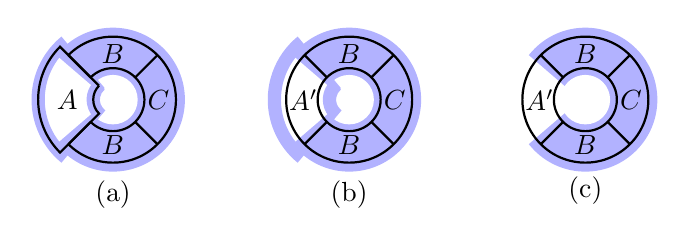
\begin{tikzpicture}[every path/.style={thick}, scale=0.4]
\begin{scope}[xshift=-7.5cm]
		 \filldraw[blue!30!white] (0,0) circle (2.25cm);
	\filldraw[white] (0,0) circle (0.75cm);
	\filldraw[white] (150:0.75cm) -- (142.5:2.5cm) -- (142.5:2.5cm) arc (142.5:217.5:2.5cm) -- (210:0.75cm) -- (210:0.75cm) arc (210:150:0.75cm) --cycle; 
	
	\filldraw[blue!30!white] (130:0.45) -- (130:0.8) arc (130:230:0.8) -- (230:0.45) arc (230:130:0.45);
	\filldraw[blue!30!white] (130:2.2) -- (130:2.55) arc (130:230:2.55) -- (230:2.2) arc (230:130:2.2);
	
	\draw[] (135:0.625) -- (135:2.375) arc (135:225:2.375) -- (225:0.625) arc (225:135:0.625);
    \draw[] (135:1) arc (135:-135:1);
    \draw[] (135:2) arc (135:-135:2);    
    
    \draw (45:1) -- (45:2);
    \draw (135:1) -- (135:2);
    \draw (-135:1) -- (-135:2);
    \draw (-45:1) -- (-45:2);
    
    \draw (0:1.45) node{$C$};
    \draw (90:1.45) node{$B$};
    \draw (180:1.45) node{$A$};
    \draw (270:1.45) node{$B$};
		
		\node[] () at (0, -3cm) {(a)};
\end{scope}
\begin{scope}
    \filldraw[blue!30!white] (0,0) circle (2.25cm);
	\filldraw[white] (0,0) circle (0.75cm);
	\filldraw[white] (150:0.75cm) -- (142.5:2.5cm) -- (142.5:2.5cm) arc (142.5:217.5:2.5cm) -- (210:0.75cm) -- (210:0.75cm) arc (210:150:0.75cm) --cycle; 
	
	\filldraw[blue!30!white] (130:0.45) -- (130:0.8) arc (130:230:0.8) -- (230:0.45) arc (230:130:0.45);
	\filldraw[blue!30!white] (130:2.2) -- (130:2.55) arc (130:230:2.55) -- (230:2.2) arc (230:130:2.2);
	
    \draw (0,0) circle (1cm);
    \draw (0,0) circle (2cm);
    
    \draw (45:1) -- (45:2);
    \draw (135:1) -- (135:2);
    \draw (-135:1) -- (-135:2);
    \draw (-45:1) -- (-45:2);
    
    \draw (0:1.45) node{$C$};
    \draw (90:1.45) node{$B$};
    \draw (180:1.45) node{$A'$};
    \draw (270:1.45) node{$B$};
				\node[] () at (0, -3cm) {(b)};
\end{scope}
\begin{scope}[xshift=7.5cm]
		\filldraw[blue!30!white] (0,0) circle (2.25cm);
	\filldraw[white] (0,0) circle (0.75cm);
		\filldraw[white] (150:0.75cm) -- (142.5:2.5cm) -- (142.5:2.5cm) arc (142.5:217.5:2.5cm) -- (210:0.75cm) -- (210:0.75cm) arc (210:150:0.75cm) --cycle; 
    \draw (0,0) circle (1cm);
    \draw (0,0) circle (2cm);
    
    \draw (45:1) -- (45:2);
    \draw (135:1) -- (135:2);
    \draw (-135:1) -- (-135:2);
    \draw (-45:1) -- (-45:2);
    
    \draw (0:1.45) node{$C$};
    \draw (90:1.45) node{$B$};
    \draw (180:1.45) node{$A'$};
    \draw (270:1.45) node{$B$};
        \node[] () at (0, -2.875) {(c)};
\end{scope}
\end{tikzpicture}

\end{document}